\chapter{Web API} 
\label{ch:Chapter4}
\vfill \minitoc \newpage

\noindent 

The web API follows a \gls{rest} approach over \gls{http} which allows for a standardized and scalable architecture for building robust and interoperable systems.

The REST API offers 1) Simplicity - as it leverages existing HTTP methods and status codes, making it easy to understand. 2) Scalability - designed to be stateless, meaning each request contains all the necessary information to be processed independently. This allows for horizontal scaling so we can add more servers to handle increased traffic without impacting the functionality of the API. 3) Flexibility - Uses JSON format for responses, which is widely supported and easy to parse in various programming languages. This flexibility makes it easier for clients to consume the API and integrate it into their applications.

In the current version of the API a overview of the endpoints is represented in Figure~\ref{fig:Endpoints}.


\begin{figure}[!ht]
	\centering
	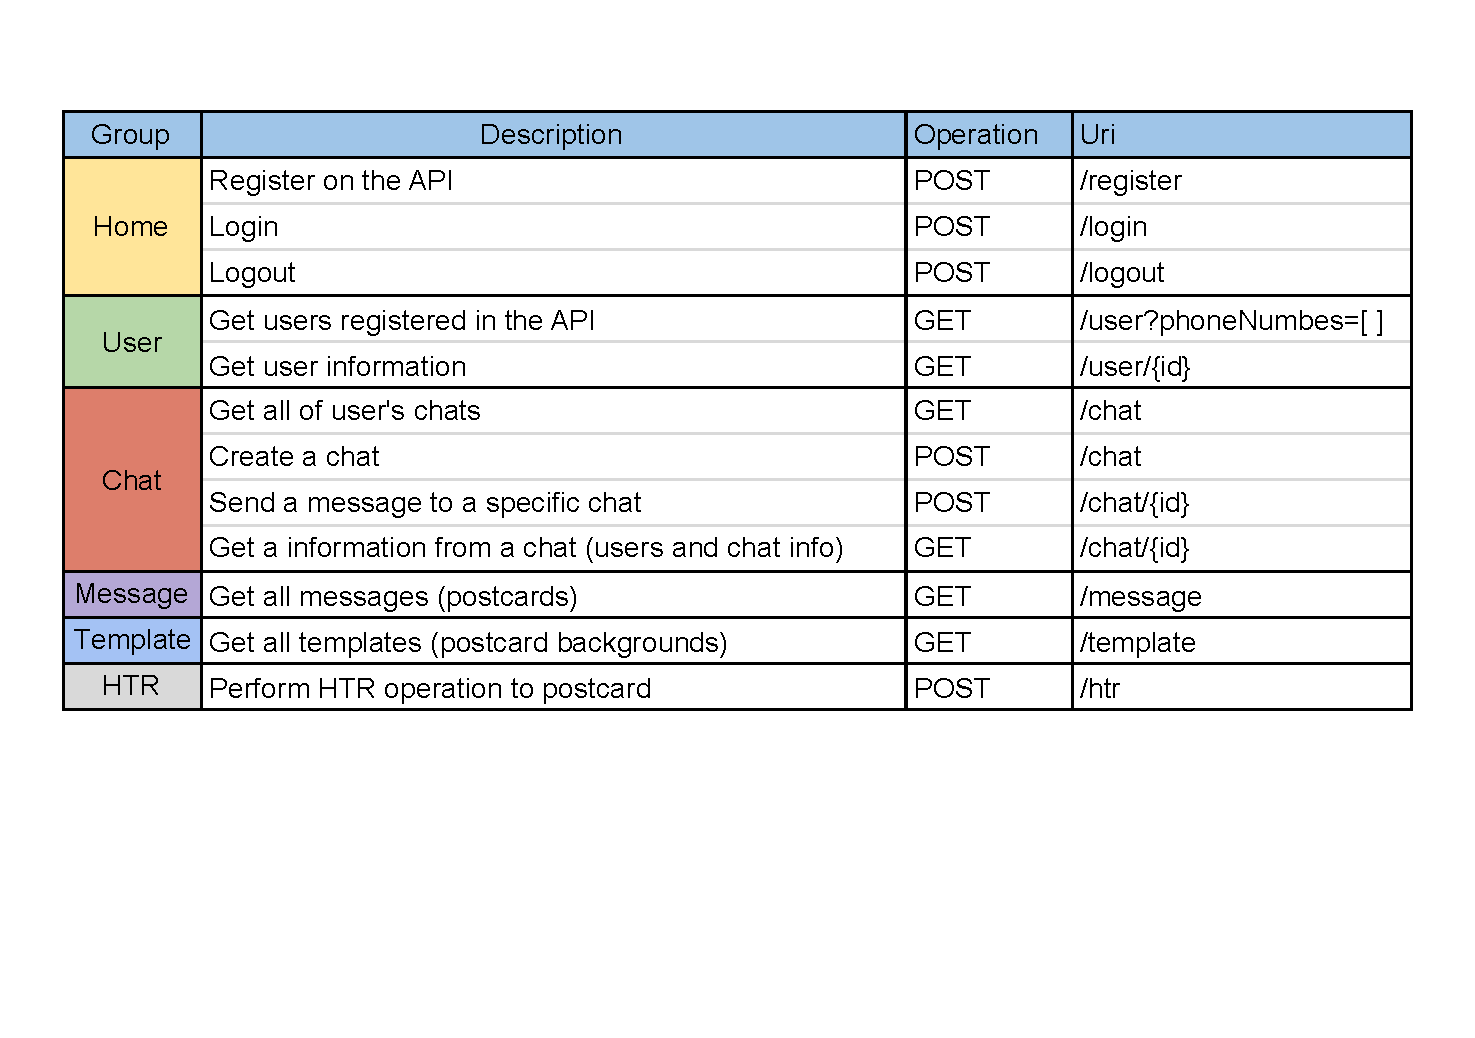
\includegraphics[trim={0cm 4cm 0cm 0cm}, width=1\textwidth]{./Chapter4/Figures/API_Endpoints}
	\caption{PostChat API endpoints.}
	\label{fig:Endpoints}
\end{figure}


\newpage


\section{Implementation}

\paragraph{Structure}

The API uses Spring MVC framework, is written in kotlin and runs in the JVM.
The structure of the API is described in Figure~\ref{fig:Structure}

\begin{figure}[!ht]
	\centering
	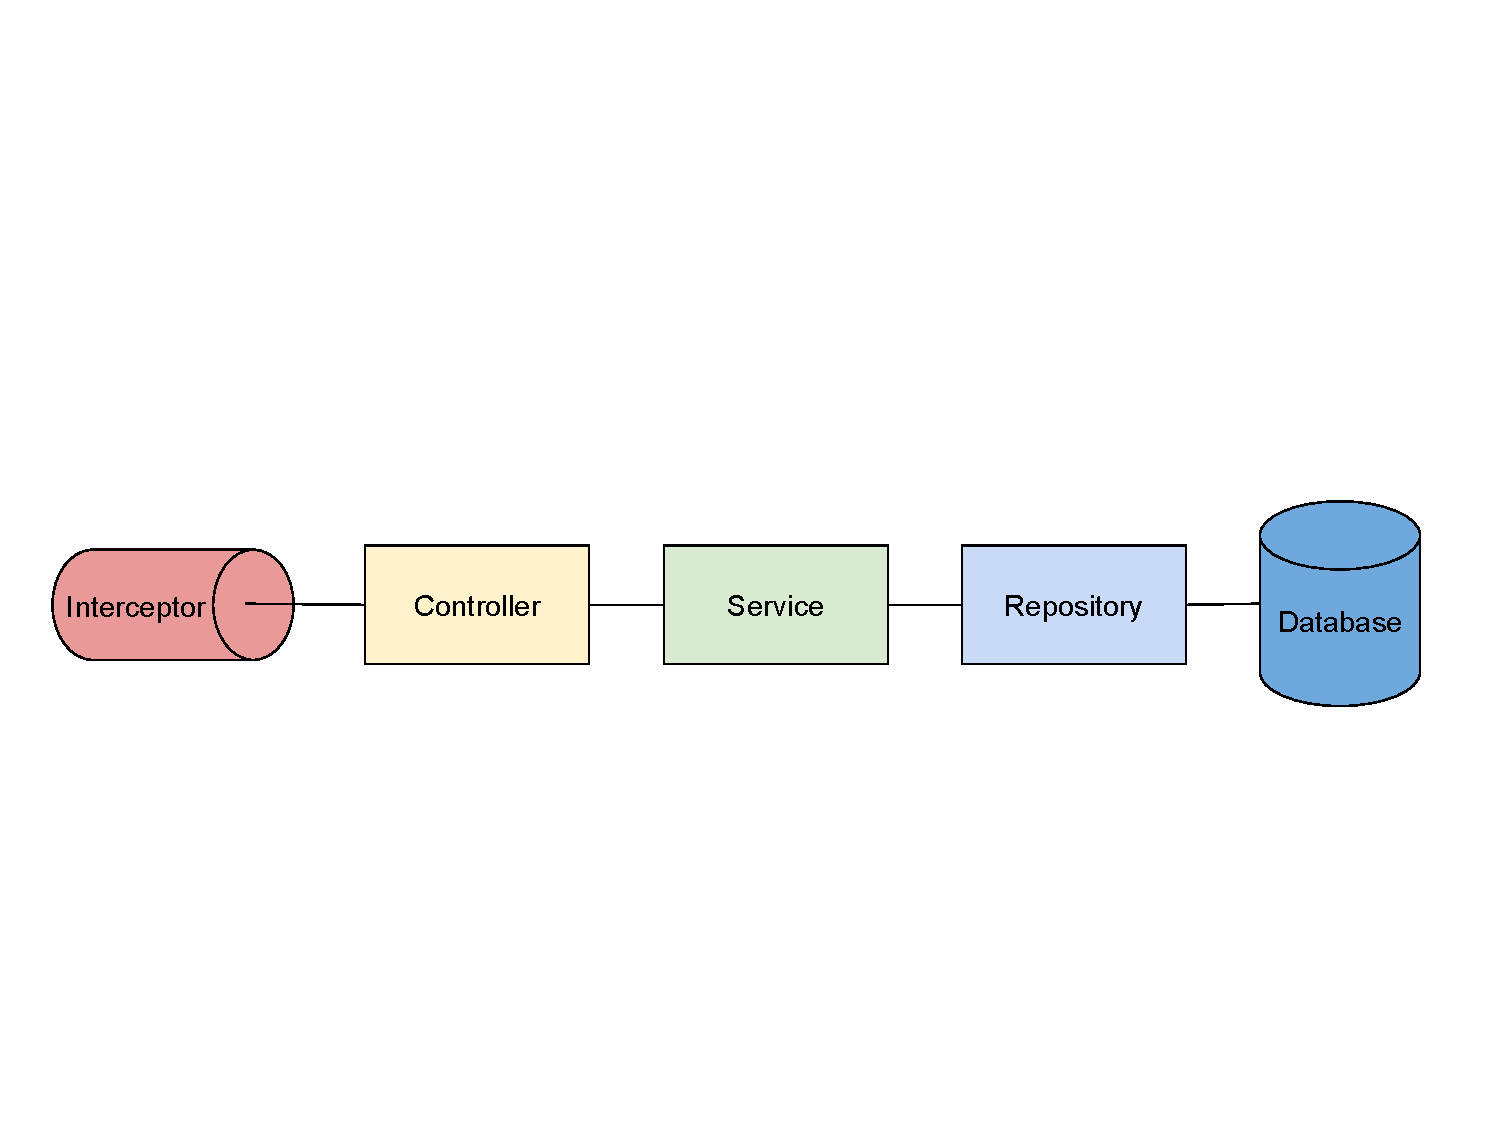
\includegraphics[trim={0cm 7cm 0cm 7cm}, width=1\textwidth]{./Chapter4/Figures/API Structure}
	\caption{API Structure.}
	\label{fig:Structure}
\end{figure}

Spring simplifies the process of implementing a Web API by providing a comprehensive and feature-rich framework that abstracts away much of the complexity associated with building APIs. The main benefits of using Spring in this project are:
\begin{itemize}
    \item Dependency Injection: Spring's dependency injection (DI) container allows for easy management and wiring of components within the API. By leveraging DI, developers can declaratively define and inject dependencies into their API classes, promoting loose coupling and enhancing testability.

    \item Inversion of Control (IoC): Spring's IoC container takes care of instantiating and managing the lifecycle of API components, relieving developers from manually managing object creation and destruction. This simplifies the development process and helps maintain a consistent and predictable application state.

    \item Annotation-driven Development: Spring encourages the use of annotations for defining API endpoints, mapping request methods, and handling request parameters.

    \item Exception Handling: Spring offers robust exception handling mechanisms, allowing developers to define custom exception handlers that gracefully handle and transform exceptions into appropriate HTTP responses. This simplifies the process of handling errors and communicating meaningful error messages to API clients.

    \item Security and Authentication: Spring Security offers a comprehensive set of features for implementing authentication and authorization mechanisms in an API. It provides declarative security configurations, authentication providers, and authorization rules, simplifying the implementation of secure APIs.

\end{itemize}

A request flow is defined in the Figure~\ref{fig:Structure} in order from left to right.

\subsection{Profiles}
Spring Profiles are used to simplify configuring the API for production and testing. Several components are annotated with 
\textit{Profile(<profile name>)} which determines what component to use for each profile.
One good use for the Profiles is to determine which database source to use depending on the profile name chosen (for production or testing).

\subsection{Interceptors}
An interceptor is a component that has the ability to intercept and process requests and responses, it provides a way to customize the behavior of the request/response processing pipeline. In the PostChat API three interceptors are implemented:

\begin{itemize}
        \item Logger Interceptor - The logger interceptor is used for every request/response, it's use is mainly for logging and debug. For every request, a entry is logged containing information about the request's method and URI and the response's status code;
        \item Content Interceptor - The content interceptor guaranties that every request body has application-json Content-Type;
        \item Authentication Interceptor - The authentication interceptor is a crucial part of the API it automates the authentication process by parsing and verifying the token cookie or the Bearer-Token header.
\end{itemize}

\subsubsection{Authentication Interceptor}
The server generates a session token when login-in or registering. The function of the authentication interceptor is to verify this token.
The authentication interceptor intercepts every request that is processed by a handler containing a parameter annotated by the \textit{Authenticate} java annotation.
Figure~\ref{fig:Interceptor Structure} illustrates a request needing authentication.

\begin{figure}[!ht]
	\centering
	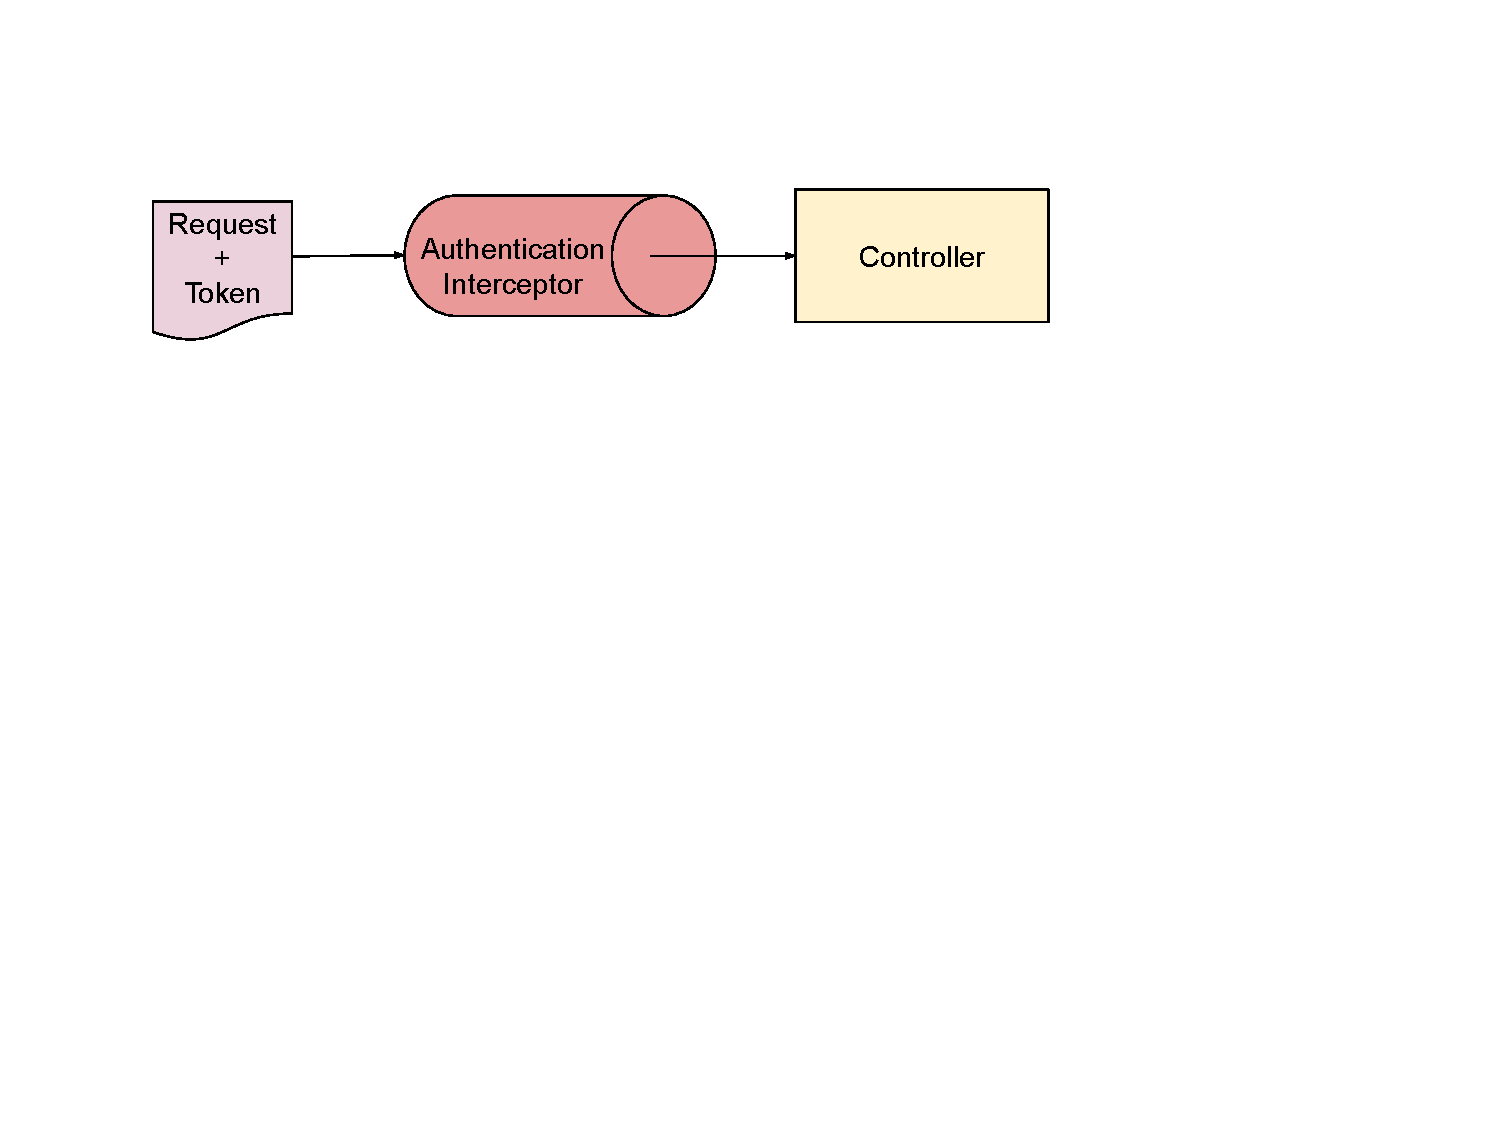
\includegraphics[trim={0cm 12cm 5cm 2cm}, width=1\textwidth]{./Chapter4/Figures/Interceptor Structure}
	\caption{Authentication Interceptor.}
	\label{fig:Interceptor Structure}
\end{figure}



A handler having a parameter annotated by the \textit{Authenticate} is marked for an authenticated operation, that is, only users signed in the application are supposed to use these operations, an implementation of the annotation and a controller handler is shown below.

\begin{verbatim}
@Target(AnnotationTarget.VALUE_PARAMETER)
annotation class Authenticate
\end{verbatim}


\begin{verbatim}
@GetMapping
@ResponseStatus(HttpStatus.OK)
fun getChats(@Authenticate user: User): ChatList =
    service.getChats(user.phoneNumber)
\end{verbatim}
 

\subsection{Controllers}
A controller is a key component in Spring MVC that plays a crucial role in handling HTTP requests and generating appropriate responses. Acting as the middleware between the user interface and the business logic (service), the controller facilitates the flow of data and interactions within the web application.

A controller class encapsulates a collection of handler methods, each of which defines a specific HTTP operation (such as GET, POST, PUT, DELETE) and its corresponding URI. These handler methods are responsible for processing the incoming requests and executing the necessary business logic.

By mapping URLs and HTTP methods to the appropriate handler methods, the controller determines which code should be executed to handle a particular request. This mapping is typically defined using annotations like @RequestMapping, @GetMapping, @PostMapping, etc., which allow developers to specify the desired URL patterns and HTTP methods for each handler method.

\subsection{Services}
Services refer to the components responsible for implementing the business logic and functionality required to fulfill the API's purpose. 
Services encapsulate specific operations and actions that can be performed on the data.

Services contain the implementation of the business logic that defines how the API handles and processes requests. They encapsulate the specific operations, algorithms, and rules necessary to perform the desired functionality. 

Services interact with the database to retrieve, modify, or persist data required by the API. They may encapsulate data access logic and perform CRUD (Create, Read, Update, Delete) operations on the underlying data. Are responsible for handling data validation, transformation, and manipulation to ensure data integrity and consistency.
The interaction with the database is done using JDBI, which is a top level implementation of the JDBC library.

For input data validation that doesn't require database operations, a object \textit{Check} was implemented. Every method defined in the object was implemented following a blockchain pattern, that is, every method return a reference to the same object leading to the ability to call successive methods in a chain.     

\subsection{Repository}
A repository is a component that encapsulates the logic for interacting with data storage systems, such as databases, file systems, or external services. It provides a set of methods and operations to perform common data operations, such as retrieving, creating, updating, and deleting entities. The primary purpose of a repository is to abstract the complexities of data access and provide a clean, domain-specific interface for the business logic to interact with the data.

The repository component abstracts the underlying data storage by providing a consistent and unified interface. It shields the business logic from the specifics of the data storage system, such as the query language or the data access technology being used. By encapsulating data access logic within the repository, it promotes modular and reusable code, allowing the business logic to be decoupled from the implementation details of the data storage.

Repository offers a set of standard data access operations, such as querying entities based on specific criteria, inserting new entities, updating existing entities, and deleting entities from the data storage. These operations are implemented within the repository, utilizing appropriate data access technologies and SQL queries, to interact with the data storage efficiently. By providing a consistent interface for these operations, the repository simplifies the implementation of data access and persistence logic.

Queries were written in raw format so all information about a specific query can be found in the method that implements the repository operation.



\subsection{Transaction Manager}
For database operations a transaction manager is defined. A transaction manager, as the name suggests, manages transactions made in the repository component by encapsulating instances of the repositories and exposing them to the Service in a lambda function. It automatically closes and opens connections to the database. The Figure~\ref{fig:TManager} illustrates how the transaction manager works. 

\begin{figure}[!ht]
	\centering
	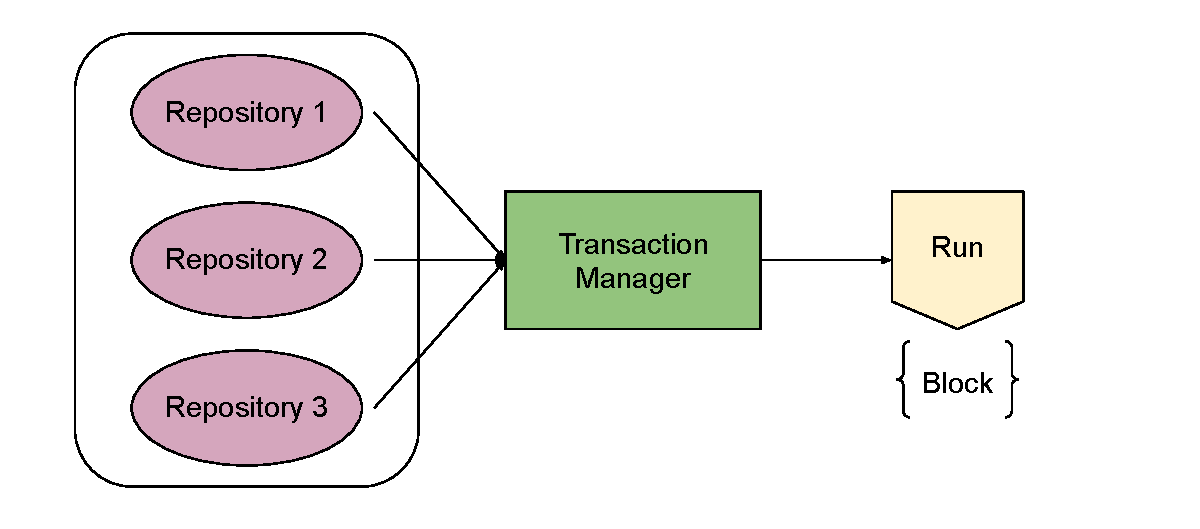
\includegraphics[width=1\textwidth]{./Chapter4/Figures/TManager}
	\caption{Transaction Manager.}
	\label{fig:TManager}
\end{figure}

The transaction manager receives the services instances and passes transaction handlers to it. The manager offers a singular method called \textit{run}, this method exposes the repositories and encapsulates the transaction.

\newpage

\subsection{Error Handling}
Errors are handled in the application by using a \textit{ControllerAdvice} annotated class called \textit{ErrorHandler}.

There are API specific defined Exceptions that are thrown when an error occurs.
The error responses are returned in a body with application/problem+json Content-Type.

The \textit{ControllerAdvice} annotation is used to define a global exception handler. This class plays a crucial role in centralizing the error handling logic across multiple controllers within the application. It intercepts and handles exceptions that occur during request processing, providing a consistent approach to handling errors.


The ErrorHandler has a method called \textit{handleException} that is annotated with @ExceptionHandler(Exception::class), indicating that it is responsible for handling any uncaught exceptions that occur within the application. This method takes the exception as an argument and returns a ResponseEntity wrapping a ProblemJSON object.

For any other unhandled exceptions, a default response entity is created with an internal server error status code and a problem type detail that includes the exception message. This generic error handling ensures that unexpected exceptions are appropriately handled, preventing the exposure of sensitive information to API clients.

By utilizing the @ControllerAdvice annotation and implementing a centralized error handling approach, this code enhances the robustness and reliability of the web API. It ensures consistent error responses across all controllers, simplifies exception handling logic, and promotes maintainability of the application. Additionally, the logging of exceptions aids in debugging and monitoring the application's health.

\section{Postcard}
A postcard is represented as a combination of layers:
\begin{itemize}
    \item Handwritten content - Represents the text (paths) drawn by the user as a SVG encoded in a base 64 string.
    \item Template - Represents a postcard background as a SVG encoded in a base 64 string. 
\end{itemize}

This approach contributes for smaller sized SVG's when sending a message and improved results from the Detector in the AI pipeline.  

\bigskip
\bigskip
\begin{figure}[!ht]
	\centering
	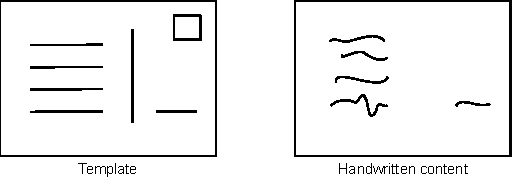
\includegraphics[width=0.6\textwidth]{./Chapter4/Figures/Postcard Representation}
	\caption{Postcard Representation.}
	\label{fig:Postcard Representation}
\end{figure}


\subsection{Message}
\label{subsec:Message}
A message is a data structure that connects a postcard to a chat element. It is the holder of the postcard information and contains all necessary information to perform further operations in the API.
Its composition is:
\begin{itemize}
    \item The phone number of the user that sent the postcard;
    \item The message id; 
    \item The chat id;
    \item The handwritten content;
    \item The merged content \ref{subsec:SVGManipulation};
    \item The template name;
    \item The timestamp of when it was created.
\end{itemize}


\subsection{Messaging Flow}
After creating a chat user can now send a postcard, to send a postcard there are three things needed 1) the name (identifier) of the template used, 2) the handwritten SVG in base 64 string and 3) the timestamp of when it was sent.
The Figure~\ref{fig:PSENDFlow} illustrates the messaging send flow.

\bigskip
\bigskip


\begin{figure}[!ht]
	\centering
	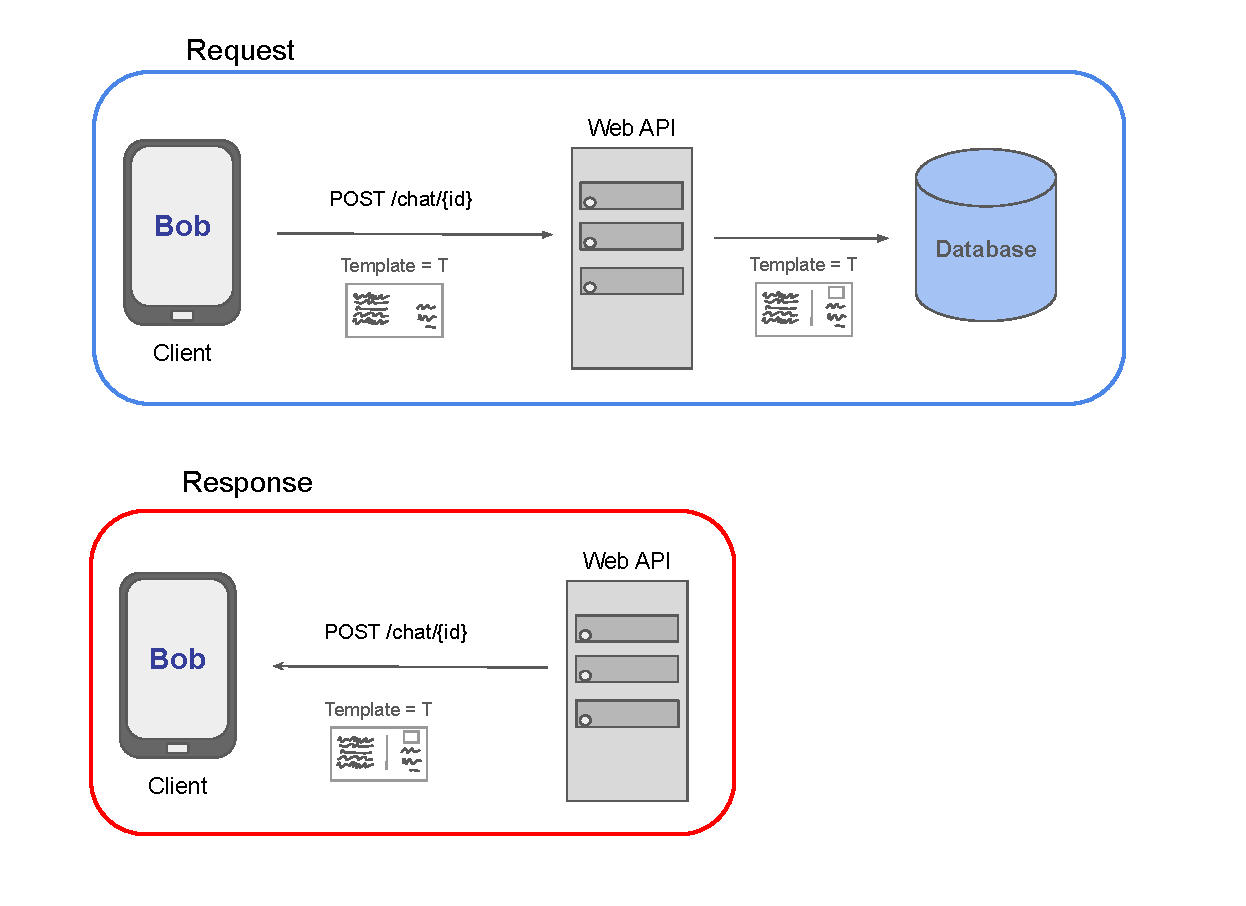
\includegraphics[trim={0cm 0cm 0cm 0cm}, width=1.1\textwidth]{./Chapter4/Figures/Postcard POST Flow}
	\caption{Postcard POST Flow}
	\label{fig:PSENDFlow}
\end{figure}

\bigskip
\bigskip
\bigskip

The server responds back with a body containing the saved message.  The same response body applies for the list of messages when getting all messages.  


\paragraph{Getting all messages} Messages are defined in a different URI from Chats, the reason of that is because we want to get all the messages across all chats, so to make a concise URI definition the Message URI was added (look into Figure~\ref{fig:Endpoints} for all endpoints).
Figure~\ref{fig:PGETFlow} illustrates getting all messages.

\begin{figure}[!ht]
	\centering
	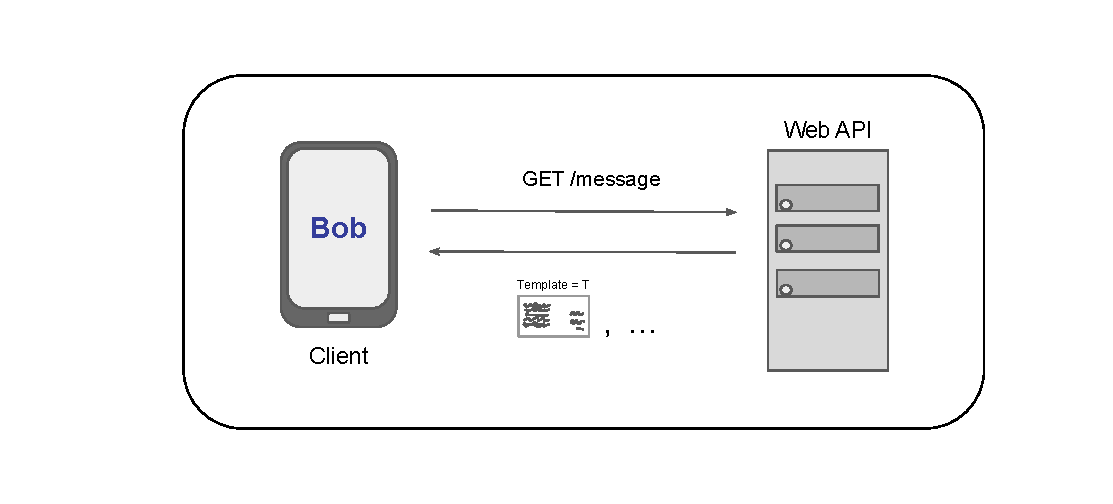
\includegraphics[width=1\textwidth]{./Chapter4/Figures/Postcard GET Flow}
	\caption{Postcard GET Flow}
	\label{fig:PGETFlow}
\end{figure}

As soon as the user receives all pending messages, the same are delete from the server's database and can no longer be retrieved. 

\bigskip
\bigskip
\bigskip


\subsection{SVG Manipulation}
\label{subsec:SVGManipulation}
When retrieving a message we want to keep it simple for any front end application to display the postcard, for that reason the template and the the handwritten content are merged into one new \gls{svg} document and encoded into base 64. Figure~\ref{fig:SVGMerge} illustrates the merging process of a \gls{svg}

\begin{figure}[!ht]
	\centering
	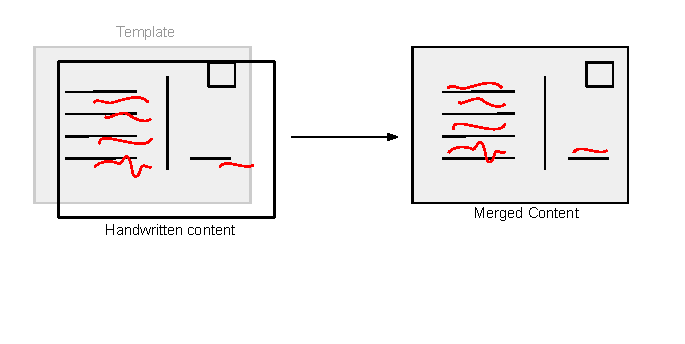
\includegraphics[trim={ 0cm 1,5cm 0cm 0cm },width=1\textwidth]{./Chapter4/Figures/Svg Merging}
	\caption{SVG Merging}
	\label{fig:SVGMerge}
\end{figure}


\newpage

\section{Database Representation}
Database uses PostgreSQL, an open-source relational database management system (\gls{rdbms}) known for its reliability, robustness, and extensive feature set.
The database EA model can be found in Figure~\ref{fig:EA}


\begin{figure}[!ht]
	\centering
	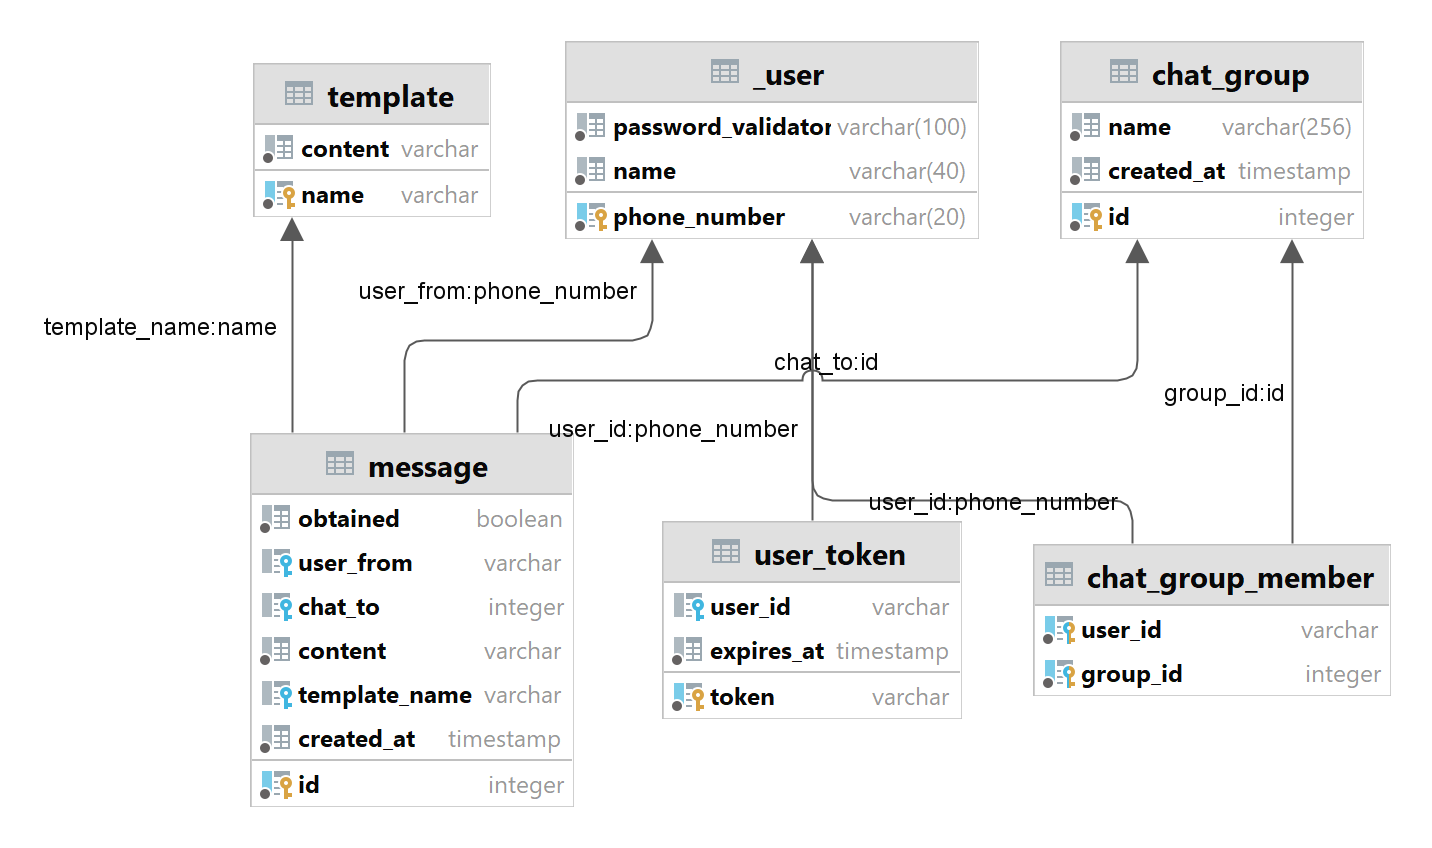
\includegraphics[trim={ 0cm 0cm 0cm 0cm },width=0.9\textwidth]{./Chapter4/Figures/EA}
	\caption{Entity Association Model}
	\label{fig:EA}
\end{figure}

Notice that \textit{ chat\_group\_member } is what defines the relation between a Chat and a User, as it is a many to many relation, and that its key is defined by the User's identifier plus the Group's identifier.

Templates are relatively small sized SVG's (normally never exceeding the KB's region) and so the same are saved in the database as a base 64 encoded string.

Message's \textit{ obtained } works as a flag to allow the message to be later removed.   

\section{Application Runner and Storing Templates}

\paragraph{Application Runner}
In Spring Framework, an ApplicationRunner is an interface that allows us to perform certain tasks after the Spring Boot application has started. It provides a convenient way to execute code logic that needs to run during the initialization phase of the application.

\paragraph{Storing Templates}
In order to automatically add templates to the database a Spring element \textit{ RunnerInsertTemplates } is defined, it implements the \textit{ ApplicationRunner } interface. When running the server the \textit{ RunnerInsertTemplates } will search for files in a specified \textit{templates} folder and automatically insert all new templates.
It is important to say that the templates names must be unique as it is the identifier for the database.

\section{Verifying Phone Numbers}
Verifying phone numbers is an important aspect of many applications and services to ensure the accuracy and legitimacy of user-provided contact information. While the implementation of SMS phone verification is not currently available, the application utilizes Google's Libphonenumber library for phone number validation.

The Libphonenumber library is a widely used and trusted library for working with phone numbers. It provides functionality to parse, format, and validate phone numbers based on international standards and regional conventions. By utilizing this library, the application can perform various operations related to phone numbers, such as extracting the country code, validating the number's format, and determining the type of phone number (e.g., mobile, landline).

Although \gls{sms} phone verification is not yet implemented, the Libphonenumber library offers valuable features to ensure that the provided phone numbers are in a valid format and conform to the expected structure. This helps in reducing errors and preventing the submission of incorrect or invalid phone numbers.

When verifying phone numbers using the Libphonenumber library, the application can perform checks such as validating the length, format, and potential existence of the number. However, it's important to note that the library's validation does not guarantee the actual ownership or availability of the phone number, as it primarily focuses on the technical aspects of number validation.

To implement \gls{sms} phone verification in the future, the application would need to integrate with a suitable \gls{sms} gateway or service provider that can send verification codes to the provided phone numbers and handle the verification process. This additional functionality would allow the application to send \gls{sms} messages containing verification codes and verify them against user-provided inputs.


\section{Performing HTR}

\noindent

Because our \gls{htr} model is written in python, the source code folder must be known by the server. The \textit{PYTOOLS\_POSTCHAT} environment variable should be defined and must contain the absolute path to the python source folder.

Our python model takes a \gls{png} file as input therefore the \gls{svg} content needs to be converted to a temporary \gls{png} file, this is done by using Apache's Batik Image converter.

The HTR operation is performed by the \textit{htr} method. It takes the handwritten content encoded in base 64 as input and returns the recognized text as a String.

In order o perform such operation the server needs to call python code, to do so, it uses Java's \textit{ProcessBuilder}. 

The \textit{ProcessBuilder} takes \textbf{"python", "main.py", "--source", <png file path>} as the program arguments and the source folder as default directory, we then proceed to start the process and wait (in a separate thread) for the process to finish. When done it will print in the standard output the recognized text, we then catch that output and return it.
